\documentclass[a4paper,twoside]{article}
% Official class, fonts, layout and bibliography style are used unchanged.
\usepackage{epsfig}
\usepackage{subcaption}
\usepackage{calc}
\usepackage{amssymb,amstext,amsmath,amsthm}
\usepackage{multicol}
\usepackage{pslatex}
\usepackage{apalike}
\usepackage{algorithm2e}
\usepackage[bottom]{footmisc}
\usepackage[T1]{fontenc}
\usepackage[utf8]{inputenc}
\usepackage{graphicx,booktabs,array,tabularx,url}
\usepackage{tikz}
\usetikzlibrary{arrows.meta,positioning}
\usepackage[hidelinks]{hyperref}
\usepackage{SCITEPRESS}
\newcolumntype{Y}{>{\raggedright\arraybackslash}X}
\newcommand{\bits}{\operatorname{bits}}
\newcommand{\rank}{\operatorname{rank}}
\newcommand{\aifootnote}{\footnote{Drafting used Codex \cite{codex}. See the disclosure.}}
\newlength{\pubtablewidth}
\setlength{\pubtablewidth}{\textwidth}


\hypersetup{pdftitle={Exact Bidirectional Steganographic Transport with Language and Pixel Autoregressive Models},pdfauthor={},pdfsubject={Anonymous regular paper, Artificial Intelligence},pdfkeywords={Generative steganography, artifact recovery, autoregressive models}}
\begin{document}
\title{Exact Bidirectional Steganographic Transport with Language and Pixel Autoregressive Models}
\author{}
\keywords{Generative Steganography, Autoregressive Models, Exact Recovery, Steganalysis, GPU Inference.}
\abstract{Generative steganography must survive the serialization of a model's decisions into a delivered file. We develop a shared authenticated packet protocol for hiding canonical grayscale images in generated text and literal UTF-8 messages in generated PNGs, with recovery by an independent receiver using only the saved artifact and shared configuration, context and key. A controlled comparison of fixed-rank, entropy-gated and arithmetic coding uses a language model and a pixel autoregressive model under the same packet and modality-specific carrier limits. Across 120 held-out transmissions, fixed and gated coding each recover 20/20 payloads in both directions. Arithmetic coding recovers 20/20 PNG payloads but 0/20 text payloads because the generated trajectories provide insufficient information before the token cap. Known-model detection exposes substantial distributional differences. Rescoring the same PNGs with one frozen alternate conditioning row reduces fixed-rank mean-surprisal AUC from 0.8850 to 0.6975, without establishing secrecy. Finally, CUDA graph replay reduces matched development encode-plus-decode latency by 5.13 times while preserving checked probabilities, carrier bytes and recovery. These results connect exact artifact transport, finite capacity, observer knowledge and practical execution cost.}
\onecolumn\maketitle\normalsize\setcounter{footnote}{0}\vfill
\section{\uppercase{Introduction}}
\label{sec:introduction}
Autoregressive models carry information through choices made during generation. A language model can select a token according to a hidden symbol, and a pixel model can do the same with a channel value. The receiver must recover the intended bytes from the object actually delivered. A text file does not preserve token identifiers, and a PNG contains pixels rather than the sender's latent state or probability trace.\aifootnote

Calgacus proposes cross-domain rank transfer, RankCloak develops bounded byte coding and entropy gating, and Pixel-Stega carries bits through autoregressive images \cite{calgacus,rankcloak,pixelstega}. We connect these foundations through a common authenticated protocol for bidirectional recovery from saved artifacts. This makes coding, serialization and finite capacity jointly testable across text and pixel models.

Our framework transports canonical images or literal messages in the same fixed-size encrypted packet within each payload group. Text generation enforces complete-prefix tokenization consistency. Image generation uses the discrete conditional probabilities of observable RGB values. Fresh receivers reconstruct model state from saved files, and a separate evaluator checks source-byte equality. Under this contract, we compare fixed-rank, gated and arithmetic coding, measure detection with a declared observer, and test one conditioning mismatch by rescoring the same PNGs. Exact probability-stream and output comparisons then establish a GPU execution improvement.

The prospective study comprises 20 held-out payload groups per direction and three methods, giving 120 transmissions. Fixed and gated coding recover every payload. Arithmetic A1 recovers all PNG payloads but accumulates insufficient information for any complete text packet under the 2,048-token cap. A matched development benchmark reduces image encode-plus-decode latency from 177.82 to 34.64 seconds while preserving the tested outputs. Together, the shared protocol and controlled comparisons explain how artifact reconstruction, distributional change and execution cost determine practical generative transport.

\section{\uppercase{Related Work}}
\label{sec:related}
\subsection{Distributional and Rank-Based Coding}
Neural linguistic steganography uses an autoregressive distribution as an information-bearing alphabet. Neural Linguistic Steganography \cite{ziegler} encodes a message through arithmetic decoding and recovers it by replaying arithmetic encoding. That work connects information efficiency to the model's conditional distributions. Our comparator follows that approach with an explicitly identified finite-message adaptation.\aifootnote

Distribution preservation is a stronger objective than recovering a packet or producing fluent text. The coupling formulation \cite{coupling} characterizes perfectly secure procedures through couplings and evaluates minimum entropy coupling on language, audio and Image Transformer channels. More recent work \cite{range} proposes rotation-based range coding with distribution-preservation guarantees and high entropy utilization. These distribution-preserving methods were not experimentally matched here. Our results establish neither superiority to them nor a limitation of every arithmetic or range coder.

Calgacus \cite{calgacus} instead transfers each payload token's context-dependent rank to a cover context. It discusses separate models, different vocabulary sizes and other discrete domains. RankCloak \cite{rankcloak} adapts rank transport to serialized cryptographic artifacts and implements bounded byte coding and entropy gating. Its repository manuscript reports 6,480 recoveries with preserved token sequences, but 88/144 recoveries in a rendered-text robustness subset. These are prior reported results, not reruns or matched baselines for our study. LlmStenoExplore \cite{explore} reproduces Calgacus and investigates finite-key collisions and perturbation sensitivity. We reuse focused rank, replay and numerical practices from this line of work, while making saved-artifact recovery the primary endpoint and separating the packet key from model conditioning.

\subsection{Pixels and Tokenization}
Pixel-Stega \cite{pixelstega} is the closest image precedent. It obtains autoregressive pixel probabilities from PixelCNN++, applies finite-precision arithmetic stegosampling, and describes transmission through a lossless public channel. Its color-image formulation identifies the red channel as the embedded variable. Our contribution is not the invention of autoregressive image steganography. We implement all delivered R, G and B values as successive observable symbols, with the correct conditional mixture posteriors, and compare three coders using the same authenticated packet and cropped, shared-row canvas as in the reverse text direction. Published Pixel-Stega capacity and detector results use different allocations and cannot be ranked against our net authenticated rates.

Published stepwise verification \cite{consistency} directly addresses detokenization and retokenization inconsistency through stepwise candidate verification. We adapt this existing idea to a pinned byte-exact tokenizer and a top-256 candidate pool. Our development comparison tests the operational consequence of replacing singleton eligibility with complete-prefix consistency, while holding the other rules fixed. It adds paired evidence for this transport contract rather than claiming tokenization consistency as a new technique.

\subsection{Detectability and Execution}
Probability and rank statistics have a history in generated-text analysis. GLTR \cite{gltr}, for example, exposes model-based token statistics to support detection. Our observer does not classify human versus generated text. It distinguishes steganographic carriers from ordinary samples of the same eligible model distribution, using two frozen whole-carrier scores. The conditioning mismatch experiment further asks how those scores change when the exact image model remains known but the observer supplies a different row. It does not test an arbitrary or fully blind adversary.

CUDA graphs are established execution infrastructure \cite{pytorchgraphs}. We measure their benefit for repeated PixelCNN++ replay and verify exact coder-interface and saved-file equivalence. A faster but numerically changed distribution could reorder ranks and break recovery.



\section{\uppercase{Method}}
\label{sec:method}
\subsection{A Shared Artifact Contract}
A public profile specifies the model, observable representation, numerical rules, coder and budget. The sender seals canonical source bytes once and encodes the packet into carrier $y$. The receiver obtains only saved $y$, the profile, shared context and encryption key. Source bytes/digests, sender identifiers, ranks, packets and latent codes are excluded. Figure~\ref{fig:examples} shows both directions using the first manifest-ordered fixed-rank example in each direction. Panel A carries canonical image pixels through saved text. Panel B carries literal text through a saved PNG.\aifootnote

\begin{figure*}[t]
\centering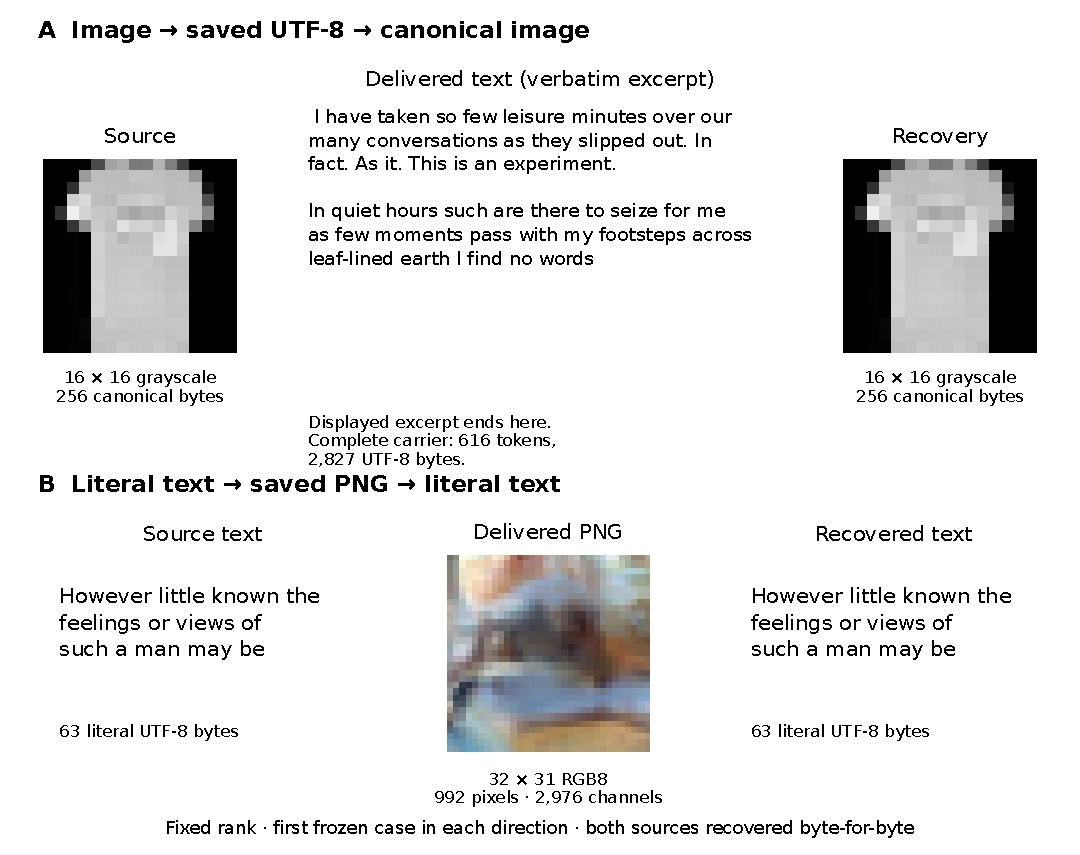
\includegraphics[width=\textwidth]{figures/figure1_transport_submission.pdf}
\caption{Actual artifacts selected by the first fixed-rank case in each direction. A transports a canonical $16\times16$ grayscale array through the displayed verbatim excerpt of a 616-token, 2,827-byte UTF-8 carrier. Recovery restores all 256 canonical pixels, not an arbitrary image file. B shows the complete 63-byte source/recovered messages and actual $32\times31$ RGB PNG. Pixels use nearest-neighbor display. Each fresh receiver uses its saved carrier, model/profile, shared context and key. The PNG conditioning row is withheld from the carrier and prepended internally. Authentication and separate source-byte equality both pass.}
\label{fig:examples}
\end{figure*}

Images are canonical $16\times16$ grayscale arrays of unsigned eight-bit pixels, 256 bytes in row-major order. Exact recovery restores this preprocessed array, not the larger original image or its container. Text is 32--128 literal UTF-8 bytes without normalization, added newlines or replacement decoding.

The plaintext header contains version (one byte, 1), kind (one byte, 1 for text or 2 for grayscale), source length (two bytes), width (two bytes) and height (two bytes). Multibyte integers are unsigned big-endian. A 256-byte slot follows, with source bytes first and zero padding. Text dimensions are zero. Image dimensions are $16\times16$. No MIME field or payload sidecar is added.

AES-256-GCM \cite{gcm} authenticates and encrypts the entire header and slot using a fresh random key and a unique random 12-byte nonce. The associated data are the exact ASCII bytes \texttt{ImageCalgacus/packet/v1}, with no newline. The carried packet is
\begin{equation}
\begin{aligned}
P&=\text{nonce}\,\|\,\text{ciphertext}\,\|\,\text{tag},\\
|P|&=12+264+16=292\ \text{bytes}.
\end{aligned}
\label{eq:packet}
\end{equation}
The known 2,336-bit target avoids circular framing around an encrypted length. After authentication the parser validates type, length, dimensions, UTF-8 and all padding bytes, returning no plaintext on failure. The evaluator checks equality separately. Authenticated encryption protects content under its usual assumptions, not the channel's existence.

One immutable packet is shared across the paired methods in a payload/context group. Reusing that ciphertext is not a new encryption under a reused nonce. Keys and nonces come from operating-system randomness, independently of sampling seeds. Continuation retains the sealed packet without supplying it to receivers.

\subsection{Observable Conditional Distributions}
At position $t$, the backend supplies eligible symbols $E_t$, normalized probabilities $q_t(v)$ and a deterministic rank order. Conditioning includes the shared context and all preceding observed symbols, including skips and completion. Text ranks use descending logits, with ascending token identifier breaking exact ties. Image ranks use descending log probability, then ascending channel value. Probability bookkeeping uses float64, stable normalization and ascending-identifier summation. NaN, positive infinity, empty support and invalid normalization are explicit failures. Numerical zero mass is excluded and the remaining distribution renormalized, without an added probability floor. Ordinary sampling is temperature-one inverse-CDF sampling in identifier order, with no nucleus truncation.

For text, the model is Llama 3 8B Instruct \cite{llama3}, not an image model. Let $T$ tokenize bytes without BOS insertion or special-token interpretation, and let $D$ return exact bytes without cleanup. Given carrier prefix $s$, each candidate $v$ must satisfy
\begin{equation}
T\bigl(D(s\mathbin{\|}[v])\bigr)=s\mathbin{\|}[v].
\label{eq:consistent}
\end{equation}
The pool contains the top 256 model tokens \emph{before} filtering. Special or control tokens, empty renderings and invalid UTF-8 are excluded. Equation~\ref{eq:consistent} is checked on the complete carrier prefix, not a prompt/carrier concatenation. The model sees one BOS followed by separately tokenized prompt bytes and carrier identifiers, without a chat template. The receiver tokenizes the delivered file separately, checks exact byte round-trip equality, and replays the same prefix tests. Payload positions, gate skips, arithmetic steps and the 32-token ordinary tail all obey this rule.

For PNG carriers, PixelCNN++ \cite{pixelcnn} models a native $32\times32$ RGB canvas. A shared $1\times32$ RGB row occupies the first row. Only the remaining 31 rows are delivered, giving 992 pixels or 2,976 channel values. Each channel value in $\{0,\ldots,255\}$ is observable. Generation and replay use raster order, with R then G then B within each pixel. The receiver reads an eight-bit RGB PNG without palette conversion, alpha compositing or color transformations and prepends the shared row internally.

The network predicts ten mixture weights, channel means, log scales and RGB dependency coefficients per pixel, not 256 independent categorical logits. Let $f_{k,C}$ denote a discretized logistic component mass for channel $C$. For normalized intensity $z(v)=2v/255-1$, component probabilities are logistic CDF differences over half-bin width $1/255$, with infinite tails at 0 and 255. Log scales are lower bounded by $-7$ and dependency coefficients use $\tanh$. We evaluate the discrete masses in float64 rather than using the upstream continuous sampler or its small-density fallback.

Channels require mixture posteriors, not independent marginals. After red, weights satisfy $w_k^R\propto w_k f_{k,R}(r)$. Green uses normalized $w^R$ and mean shift $a_{RG}z(r)$. After green, $w_k^{RG}\propto w_k^R f_{k,G}(g\mid r)$. Blue uses normalized $w^{RG}$ with mean shift $a_{RB}z(r)+a_{GB}z(g)$. One network forward per visible pixel supplies all parameters, reused within that pixel. Causal checks establish that unobserved pixels do not alter them.

\subsection{Three Packet Coders}
\label{sec:coders}
\paragraph{Fixed rank.}
Each packet byte yields its high nibble and then low nibble. A nibble $d\in\{0,\ldots,15\}$ selects eligible rank $d+1$. Exactly $292\times2=584$ positions carry the packet. The receiver inverts observed ranks into bytes and stops by this fixed count. Fewer than 16 eligible symbols while the packet is pending causes a support failure, not a smaller alphabet.

\paragraph{Entropy-gated rank.}
The same four-bit operation is applied only if
\begin{equation}
H(q_t)=-\sum_{v\in E_t}q_t(v)\log_2q_t(v)>\tau.
\end{equation}
Otherwise the sender samples ordinarily and consumes no packet bits. The receiver recomputes the strict comparison from the observed prefix, so no gate trace is transmitted. Separate thresholds were calibrated from ordinary development traces and frozen at $0.5983972524635524$ bits for text and $3.2159513527579326$ bits for channels. They were not adjusted after failures.

\paragraph{Arithmetic A1.}
We independently implement a finite-precision arithmetic comparator following Neural Linguistic Steganography \cite{ziegler}. A1 identifies our framing adaptation, not a new security construction. It starts with the half-open interval $[0,2^{32})$. At width $R$, retain symbols with $q_t(v)\geq1/R$ and at least the top $\min(2,|E_t|,R)$ symbols. Renormalize retained probabilities, round bin widths to nearest integer with ties to even, truncate before the first cumulative overflow, and assign residual width to the first symbol. Remove zero-width bins. Positive widths must sum to $R$.

The next 32 source bits, zero-extended only beyond the packet, select the interval bin. Sender and receiver emit the common leading bits of its lower bound and upper bound minus one, then shift the interval accordingly. A zero-bit step updates the interval and consumes carrier capacity. Packet completion occurs at the first common-prefix emission reaching 2,336 bits. At most 31 emitted suffix bits are checked to be zero and discarded. There is no end token, final-artifact endpoint dump or implicit flush during ordinary completion. The receiver needs no sender offset to determine progress.

This framing differs from the reference's final-token endpoint handling. A1 can stagnate when a narrow interval straddles a leading-bit boundary and quantization retains one bin, leaving that interval unchanged. Its precision and stopping rules remain fixed. Capacity exhaustion is an outcome, but desynchronization is an implementation defect. An incomplete packet prefix is not authenticated delivery.

\subsection{Stopping, Completion and Conditional Inversion}
All text carriers have a 2,048-token cap. After packet completion the sender must add exactly 32 ordinary tokens within that cap. A packet completing too late for the tail is packet-complete but carrier-incomplete. An unfinished packet is not truncated early to reserve a tail. PNG generation always completes all 2,976 channels after the packet stop, including any remainder of a partially used RGB pixel. No packet is stored in PNG metadata or appended bytes.

Inversion follows inductively when both endpoints reconstruct the same distribution and coder transition from each observed prefix. Equation~\ref{eq:consistent} supplies the text invariant, and lossless pixel equality supplies the PNG invariant. The fixed packet size supplies framing. Sufficient support and finite termination remain necessary conditions.

Senders exit before fresh receivers start. Their input directories contain only carrier, profile, context and key, with model assets separately available. Evaluation follows receiver exit. Reports distinguish packet and carrier completion, receiver recovery, authentication, carrier conformance and source equality.

\section{\uppercase{Experimental Design}}
\label{sec:design}
\subsection{Sources, Contexts and Pairing}
Development used 20 images and 20 texts with two contexts per direction. Five synthetic image fixtures were supplemented by 15 Fashion-MNIST training images. Five literal text fixtures, including non-ASCII UTF-8, were supplemented by 15 narrative spans from Gutenberg ebooks 11 and 84. Sources, canonicalization, contexts, profiles and thresholds were frozen before prospective generation.\aifootnote

The held-out image set contains 20 Fashion-MNIST test images, two per class \cite{fashion}, BOX-resized from $28\times28$ grayscale to $16\times16$. Twenty nonoverlapping text spans come from Austen's \emph{Pride and Prejudice} and Doyle's \emph{The Adventures of Sherlock Holmes}, Gutenberg ebooks 1342 and 1661. Ten messages occupy each 32--64-byte and 65--128-byte band. Observed lengths are 58--128 bytes, with mean 93.2. Snapshot hashes, source indices/byte offsets and exclusions are recorded. Boilerplate, duplicate original/canonical bytes and development/held-out overlap are excluded without using generated outcomes. Fashion-MNIST's MIT notice and Gutenberg attribution are retained. The texts are unrestricted under US copyright, not necessarily every jurisdiction.

The prospective prompt is ``Write a calm field-journal entry about a walk through a temperate forest. Use continuous prose.'' Row1 is the first row of an independently generated development image with context seed 2001. Neither context is included in the delivered carrier. Table~\ref{tab:specification} summarizes the frozen allocation.

\begin{table*}[t]
\caption{Frozen prospective specification. Dimensions are width by height. Both directions share a 292-byte packet, but carrier symbols and useful-rate units differ. One sealed packet is shared across methods within each payload/context group.}
\label{tab:specification}\centering\small
\begin{tabularx}{\textwidth}{@{}p{2.8cm}YY@{}}
\toprule
Property & Image payload in text & Text payload in PNG \\
\midrule
Canonical source & $16\times16$ grayscale, 256 raw bytes & Literal UTF-8, 32--128 bytes \\
Delivered artifact & Strict UTF-8, at most 2,048 tokens & $32\times31$ RGB8 PNG, 2,976 channels \\
Neural model & Llama 3 8B Instruct, Q4\_K\_M GGUF & CIFAR-10 pretrained PixelCNN++ \\
Runtime & llama-cpp-python 0.3.23, 33/33 CUDA layers & PyTorch 2.5.1+cu124, float32 CUDA \\
Shared context & Forest prompt, separate tokenization & Private $1\times32$ RGB row, 96 bytes \\
Eligible symbols & Top 256, then complete-prefix filtering & Discrete R/G/B values 0--255 \\
Coders & Fixed radix 16, gated radix 16, arithmetic A1 & Same coders and 2,336-bit target \\
Completion & 32 ordinary tokens after the packet & All channels through the last visible pixel \\
Payload groups & 20 held-out images, one context & 20 held-out texts, one context \\
Controls & 20 traces, matched prefixes & 20 PNGs shared across methods \\
\bottomrule
\end{tabularx}
\end{table*}

The allocation is $20\times3\times2=120$ stego units. Each payload/context group shares one immutable packet, source and model across three methods. Sampling seeds are separate from encryption randomness. Terminal failures remain observations, and continuation neither duplicates completed carriers nor replaces difficult sources.

One independent ordinary control is generated per group. Text controls extend to the group's longest realized carrier, 2,048 tokens in every prospective group, with length-matched prefixes for fixed and gated methods. PNG methods share one full image. All controls use the same eligibility and ordinary sampling rules. Thus 120 method associations are 40 independent traces. The frozen duplicate rule gives an identical control artifact one owner, the lowest ordered eligible group. No prospective duplicates or unscorable delivered carriers occurred.

\subsection{GPU Execution and Timing}
\label{sec:hardware}
All inference runs serially on one NVIDIA RTX 5000 Ada Generation GPU with 32 GB memory and driver 590.48.01. Text uses the QuantFactory Llama 3 8B Instruct Q4\_K\_M GGUF and embedded tokenizer. Explicit \texttt{n\_gpu\_layers=-1} is verified as 33/33 eligible layers offloaded, with \texttt{logits\_all=True} and batch/microbatch one. Context/KV state is reset between sequences and evaluation is incremental within a sequence. No CPU or partial-offload fallback is permitted.

PixelCNN++ uses a pretrained CIFAR-10 checkpoint with five residual blocks, 160 filters and ten mixtures. Strict loading, CUDA parameter/input placement and evaluation/inference modes are verified. The float32 network uses neither TF32 nor mixed precision. Deterministic algorithms, disabled cuDNN benchmarking, synchronous launches and fixed cuBLAS workspace are retained. Both backends have positive process-specific GPU activity evidence. Full hashes and settings are in the companion.

Prospective timings use the reference image path, not the later graph optimization. Charged latency spans child-process launch to exit, including imports, hashing/loading, occupied CPU work, inference, serialization and teardown. Encode/decode phase times exclude some overhead. CUDA events are nested within phases and are not added again. Fresh loading does not imply eviction of filesystem caches. The separate evaluator and wrapper monitoring joins are outside this boundary.

\subsection{Metrics and Grouped Uncertainty}
For $L$ source bytes and $N$ delivered symbols, exact goodput is $G=8L/N$ only for an authenticated, exact and conforming recovery, and zero otherwise. Text uses bits/token and PNG bits/channel value; multiplying the latter by three gives bits/pixel. Complete-packet rate counts 2,336 bits through the packet stop or across the full carrier. It is undefined for incomplete A1 text, whose prefix progress is reported separately.

Recovery uses two-sided 95\% Clopper--Pearson intervals, [0.8316, 1] for 20/20 and [0, 0.1684] for 0/20. These are Bernoulli working-model bounds for a small fixed allocation. Continuous quantities, AUCs and paired differences use 2,000 frozen PCG64 draws, base seed 2026090901 plus direction offset. Whole groups are resampled within image class or text-length band, carrying all methods and shared controls together. Intervals use the 2.5th and 97.5th percentiles. Boundary paired-binary comparisons additionally retain conservative bounds from 97.5\% marginal Clopper--Pearson intervals, rather than interpreting collapsed bootstrap intervals as certainty.

\subsection{Observer and Context Mismatch}
\label{sec:observer}
The observer knows the exact model, profile, eligibility and scoring rules and, initially, the correct context, but not the key or source. Its frozen whole-carrier scores are
\begin{align}
S(y;c)&=-N^{-1}\sum_t\log_2 q_t(y_t),\\
R(y;c)&=N^{-1}\sum_t\log_2\rank_t(y_t).
\end{align}
Higher always indicates stego. AUC is the probability that a stego score exceeds an ordinary score, with half weight for ties. No score orientation or threshold is selected using held-out labels. Scorable failed carriers remain included.

The extension retains correct-row scores and rescores the same 60 stego PNGs and 20 shared controls under row2. This random-RGB development row was frozen using PCG64 seed 2002, not detection outcomes. The scorer reads only PNG, profile and row and evaluates every delivered channel. Three predetermined development artifacts, fixed, A1 and ordinary PNG, first reproduced their retained scores and both available probability-stream digests. Paired AUC changes use 2,000 length-stratified draws, seed 2026090902, carrying both conditions, all methods and shared controls together. They are repeated measurements, not new transmissions. The subsequent within-artifact score-shift summaries are descriptive and post hoc, with no added tests or intervals.

\subsection{Matched Development Benchmark}
The lowest ordered development payload in each of three byte bands gives 32-, 96- and 128-byte messages under row1. Fixed rank has three matched timing repetitions per payload with alternating reference/graph order. The 32-byte case also tests gated and A1 once, giving 11 comparisons and 22 recoveries, not 11 independent payloads.

The graph path captures the unchanged PixelCNN++ forward after three warmups and replays from persistent input/output buffers. Both modes use fresh senders and receivers and the same retained packet. Equivalence requires exact eligible identifiers, ordering, float64 probabilities, PNG bytes, recovered bytes and completion outcomes. Headline speedup divides matched mean charged pair times over the nine fixed comparisons. Throughput pools recovered source bytes over both processes. No numerical tolerance is introduced.

\section{\uppercase{Results}}
\label{sec:results}
\subsection{Exact Artifact Recovery and Useful Rate}
The prospective allocation completed all 120 stego outcomes and 40 independent controls. There were 100 exact, authenticated and conforming recoveries and 20 retained A1 text capacity failures. All 280 model processes have GPU execution evidence. No source replacement, protocol retry, timeout or infrastructure failure was needed. Table~\ref{tab:outcomes} and Figure~\ref{fig:recovery} retain every attempt.\aifootnote

\begin{table*}[t]
\caption{Prospective outcomes and original reference-path runtime. Each cell has 20 attempted payload groups. Exact recovery is 20/20 with 95\% interval [83.16\%, 100\%], or 0/20 with [0\%, 16.84\%]. Phase means exclude loading and some process overhead. Charged means include both fresh processes and unsuccessful attempts. Goodput units are bits/token for text and bits/channel value for PNG.}
\label{tab:outcomes}
\centering\small
\begin{tabular}{@{}llrrrrrl@{}}
\toprule
Carrier & Method & Exact & Goodput & Encode (s) & Decode (s) & Charged (s) & Failure \\
\midrule
UTF-8 & Fixed & 20/20 & 3.3247 & 45.63 & 45.31 & 123.33 & None \\
UTF-8 & Gated & 20/20 & 3.1246 & 57.31 & 57.30 & 147.29 & None \\
UTF-8 & A1 & 0/20 & 0.0000 & 398.15 & 396.01 & 826.57 & Capacity \\
PNG & Fixed & 20/20 & 0.2505 & 85.27 & 85.31 & 178.18 & None \\
PNG & Gated & 20/20 & 0.2505 & 85.29 & 85.65 & 178.53 & None \\
PNG & A1 & 20/20 & 0.2505 & 85.59 & 85.77 & 179.01 & None \\
\bottomrule
\end{tabular}

\end{table*}

\begin{figure*}[t]
\centering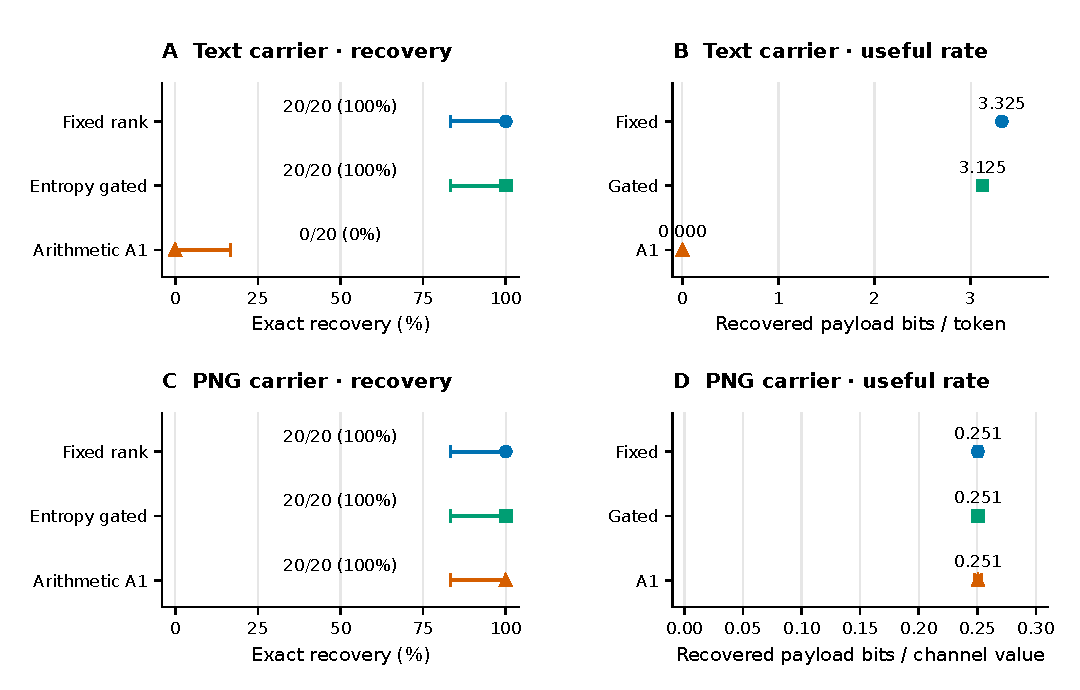
\includegraphics[width=\textwidth]{figures/figure2_recovery_rate.pdf}
\caption{Held-out recovery and exact useful rate for 20 payload groups per direction. Recovery whiskers are the accepted 95\% Clopper--Pearson bounds. Rate whiskers are the accepted stratified group-bootstrap intervals, keeping paired methods together. All failed A1 text transmissions contribute zero goodput. Text and PNG rate axes use different carrier symbols. Zero-width observed rate intervals do not imply universal reliability.}
\label{fig:recovery}
\end{figure*}

Fixed and gated coding recover 20/20 payloads in each direction. Fixed text uses 584 packet positions and 32 completion tokens, giving 3.32468 useful bits/token. Gating adds a mean 39.8 skips, reducing goodput by 0.2000 bits/token [0.1805, 0.2192] and increasing charged pair time by 23.96 seconds [20.34, 27.58]. Whole-carrier mean surprisal decreases by 0.3912 bits/token [0.3079, 0.4764].

All PNG methods recover 20/20, giving mean exact goodput of 0.25054 bits/channel [0.24731, 0.25349], or 0.75161 bits/pixel. Equal rates follow partly from the fixed full canvas and do not imply equal coder capacity. Fixed uses 584 packet channels, gating adds a mean 100.5 skips, and A1's mean packet span is 597.85 channels, including 89.65 zero-bit positions. Ordinary completion fills the remaining channels.

Framing/encryption adds 36 bytes. Texts leave a mean 162.8 padding bytes. Images fill the slot. Including completion, packet transport is 3.79221 bits/token for fixed text, mean 3.56404 for gated text, and 0.78495 bits/channel for every PNG method. A1 text has no complete-packet rate. Its PNG termination position is already included in the packet span, not an extra position.

\subsection{Arithmetic Text Reaches the Capacity Boundary}
All 20 A1 text streams reach the 2,048-token cap before producing the 2,336-bit packet. They recover between 581 and 2,216 packet-prefix bits, with mean 1,456.85. None reaches zero-extension or finite-message termination. Accordingly, none authenticates or delivers useful source bytes, despite the availability of partial information. Mean charged encode-plus-decode time is 826.57 seconds, over six times fixed text, and all that cost remains in the results.

Independent interval, partition and sender/receiver prefix checks agree with all 40 prospective arithmetic audits. Every arithmetic PNG terminates and recovers. Two failed texts have one and three isolated unchanged steps, with longest consecutive run one. A successful PNG also has one. These do not support sustained stagnation as the text-failure cause. Zero-bit steps can continue narrowing an interval without emitting a leading bit.

Cumulative surprisal closely tracks recovered text-prefix information, supporting low information under the cap rather than decoder disagreement or an unexecuted flush. This observed limit is distinct from A1's separately demonstrated stagnation case.

\subsection{Detectability with the Correct Context}
\label{sec:detection-results}


Correct-context scores show that exact recovery and low detectability are different endpoints. Both fixed and gated text have empirical mean-surprisal AUC 1.000, with bootstrap interval [1.000, 1.000]. Every observed stego score exceeds the corresponding ordinary sample range. This is complete empirical separation under the tested observer, not an assurance of perfect future detection. Failed A1 text gives AUC 0.380 [0.260, 0.503]. The below-chance orientation is retained rather than reversed to improve a detector result.

PNG scores are less separated. Fixed mean-surprisal AUC is 0.8850 [0.7425, 0.9850], gating 0.8300 [0.7000, 0.9375], and A1 0.5575 [0.3750, 0.7426]. Arithmetic PNG combines exact delivery with lower observed separation for this score, although its interval spans a wide range around chance. Every cell has 20 scorable stego artifacts and 20 unique matched controls, without exclusions. The secondary log-rank AUCs are 1.000, 1.000 and 0.360 [0.2425, 0.4801] for fixed, gated and A1 text, respectively. PNG values are 0.8400 [0.6825, 0.9650], 0.7700 [0.6299, 0.8975] and 0.5750 [0.4050, 0.7576].

\subsection{PNG Detection Depends on the Tested Context}
\begin{figure*}[t]
\centering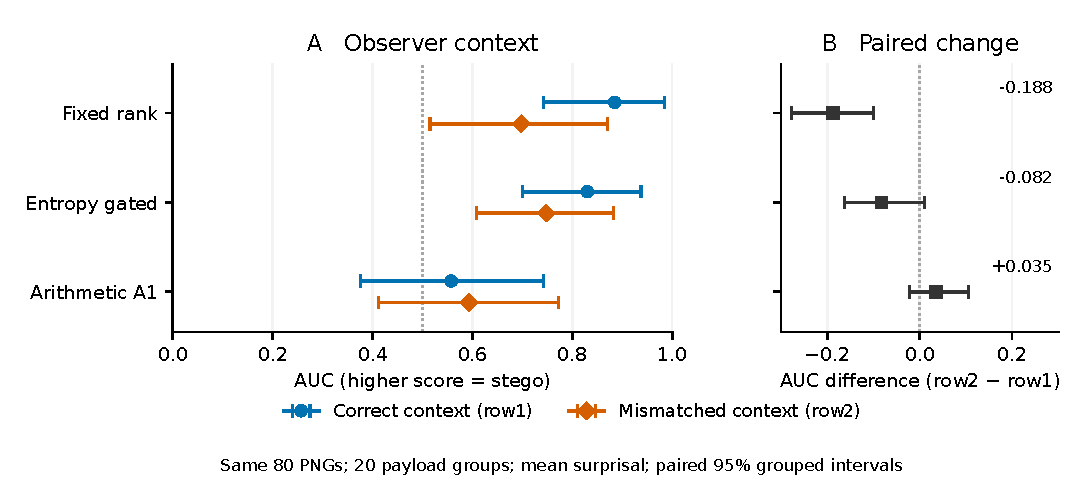
\includegraphics[width=\textwidth]{figures/context_auc.pdf}
\caption{Primary PNG detection with correct row1 and mismatched row2. The same 60 stego PNGs and 20 shared ordinary controls appear in both conditions. Panel B gives paired AUC change, row2 minus row1. Whiskers use the accepted 2,000 length-stratified group draws, jointly retaining observer conditions, methods and control ownership. The observer still knows the exact model and procedure. Row2 is the previously frozen random-RGB row, not a row selected for low detection. Reference lines are not fitted classification thresholds.}
\label{fig:png-context-auc}
\end{figure*}

All 80 retained PNGs are fully scorable under row2. Fixed-rank primary AUC decreases from 0.8850 to 0.6975, a paired change of $-0.1875$ with interval $[-0.2775,-0.1000]$ (Figure~\ref{fig:png-context-auc}). Gating changes from 0.8300 to 0.7475, or $-0.0825$ [$-0.1625$, 0.0100]. A1 changes from 0.5575 to 0.5925, or $+0.0350$ [$-0.0225$, 0.1050]. The fixed reduction is resolved by its paired interval. The gated and A1 changes remain uncertain.

Under mismatch, the primary fixed interval [0.5150, 0.8700] only narrowly excludes 0.5, and its secondary rank-score AUC is 0.6625 [0.4725, 0.8475]. The primary gated interval [0.6074, 0.8825] remains above chance. Thus this mismatch weakens the tested fixed score without removing all information from mean-surprisal detection. A resolved change for one method and an uncertain change for another do not themselves establish different method sensitivities.

Mean row2-minus-row1 score changes are 0.610 bits/channel for controls, 0.334 for fixed, 0.513 for gated and 0.629 for A1. These descriptive shifts narrow the paired fixed-minus-control gap from 0.508 to 0.231. Larger control increases are consistent with, but do not explain, the AUC change. Row1 comes from a generated image and row2 from random RGB values, so context correctness is not isolated from row statistics.

\subsection{Exact GPU Replay Improves Useful Throughput}
CUDA graph replay reduces mean fixed-rank charged encoding from 88.95 to 17.36 seconds and decoding from 88.87 to 17.28 seconds. Combined latency falls from 177.8186 to 34.6417 seconds, a matched 5.133-fold improvement. Pooled useful throughput rises from 0.4799 to 2.4633 recovered bytes per second. These nine fixed timing comparisons include both fresh processes. Gated and A1 single-payload combined times change from 180.25 to 34.61 and 182.85 to 35.11 seconds.

All 11 reference/graph comparisons preserve exact eligible identifiers, rank ordering and float64 probability streams at all 2,976 channels. All 22 PNGs recover identical source bytes, without numerical tolerance or packet rerolls. Graph replay therefore remains an explicit optional mode on this stack. It does not retroactively alter prospective timings. Peak allocated memory is 484.479 versus 473.849 MiB, reserved memory 516 versus 744 MiB and sampled process memory 912 versus 1,176 MiB for reference versus graph. These measures overlap and are not additive. PID-matched GPU activity samples are intermittent, not a sustained-utilization estimate.

\section{\uppercase{Discussion and Limitations}}
\label{sec:discussion}
The evaluated contract connects discrete model decisions to authenticated bytes recovered from files. Rank coding provides useful text capacity but a strong known-model detection signal. Arithmetic A1 recovers PNG payloads under the same packet budget, yet fails on low-information text trajectories. Practical success therefore depends on serialization, finite capacity and completion together, not nominal alphabet size alone.\aifootnote

Development isolates the serialization issue. Twenty image payloads under two prompts produce 40 packet-paired sequence/static comparisons. Complete-prefix filtering recovers 40/40, while singleton filtering recovers 22/40, split 8/20 for the forest prompt and 14/20 for the soup prompt. The 18 drift failures are literal saved artifacts, not repaired texts. This supports the main implementation's consistency requirement alongside published stepwise verification. It is not an impossibility result for alternative serializers or 40 independent payloads. Twenty lossless development PNG re-saves also preserve pixels and recover exactly through fresh processes. Neither check covers JPEG recompression, cropping or paraphrasing.

Context and key have distinct roles. The 96-byte row changes model probabilities but does not acquire cryptographic secrecy from being withheld. The specified mismatch weakens one score without testing adaptive context inference or arbitrary observers. Detecting a carrier also does not recover its encrypted source. These endpoints should not be collapsed into one security claim.

Twenty groups per direction and two pinned models define a focused allocation, not broad reliability or statistical power. Shared controls and repeated scores constrain independence. Exploratory comparisons are not family-wise confirmatory tests, and a bootstrap cannot reveal population overlap absent from a separated sample. A1 is one finite-precision adaptation, with a documented stagnation limitation and no observed complete text recovery. Its outcomes cannot be generalized to all arithmetic, range or distribution-preserving methods. Changing packet sizes, compression, contexts or caps would require another comparison.

Graph replay addresses repeated image-model launch overhead. Text filtering still consumes approximately 71\%, 75\% and 89\% of fixed, gated and A1 encoding time. Faster GPU inference cannot remove that CPU bottleneck or supply information absent under the frozen cap. The 5.13-fold result applies to three matched development payloads and the pinned reference/stack, not all prospective jobs or hardware.

Exact replay is established within the tested environment, not future libraries or GPU architectures. Third-party model and code terms still apply. The image port has a sale-restricting notice, and separate checkpoint redistribution permission was not established. No weights, keys or private row bytes are distributed with the manuscript. These are reproduction and dissemination constraints, not exceptions to the observed byte-equality endpoint.

\section{\uppercase{Conclusion}}
We develop exact bidirectional transport with a shared authenticated packet and independent recovery from saved artifacts. Fixed and gated coding recover all held-out payloads in both directions. Arithmetic A1 recovers generated PNG payloads but exposes a text capacity boundary. Known-model scores distinguish these coding choices, and a specified context mismatch changes measured PNG detectability. A development CUDA graph benchmark improves image throughput by 5.13 times while preserving checked distributions and artifacts.\aifootnote

The photograph extension reconstructs ranks from invariant cover context and recovers every evaluated packet with small bounded changes. Simple parity achieves the same recovery with slightly better mean fidelity and lower cost. The demonstrated contribution is reproducible model-rank embedding, not a learned-partition advantage. Artifact recovery, concealment and execution cost remain distinct endpoints.

\section*{\uppercase{AI Assistance Disclosure}}
\label{sec:ai}
OpenAI Codex assisted with implementation, analysis scripts, figure preparation, and drafting and editing throughout this paper and its companion \cite{codex}. Reported measurements come from retained execution records. Statistical plots display those measurements, and carrier examples are saved experimental artifacts, not AI-generated replacements. Tool assistance does not constitute independent scientific verification. Responsibility for factual accuracy, attribution and the final submission rests with the authors.
\bibliographystyle{apalike}
{\small\bibliography{references}}
\end{document}

